
For the problem of multifracturing  it is necessary to have a procedure for both integrating and interpolating the crack and pipe segments. These need arises form two reasons. 
First, when computing the fluid balance equation the volume of fractures needs to be found. Second various events of crack collisions and splits require unknown intermediate width values that must be found by interpolation the known width data on discredited grid. Three strategies for interpolation are considered. Linear, cubic and cubic Hermite splines were considered.

\paragraph{piecewise polynomial definition}

 The grid of $N$ points can be divided into $N-1$ intervals, and for each of these such values of $a_i, b_i, c_i, d_i$ are found that:

\begin{equation}\label{piecewise_polynomial}
S_i(x)=d_i(x-x_i)^3+c_i(x-x_i)^2+b_i(x-x_i)+a_i
\end{equation}

Of course in linear case for all $i$ $c_i=0$ and $d_i=0$, however the equations for evaluation of these strategies can be more easy implemented when generalized to one equation.

\paragraph{interpolation details (???)}
The details how to obtain $a_i, b_i, c_i, d_i$ could be found here



\paragraph{value evaluation}
When obtaining the value of interpolating piecewise polynomial at some point x, it is important to the interval $x_i < x\le x_{i+i}$  to locate witch  $S_i(x)$ polynomial piece to use. Then the faster too compute form of \eqref{piecewise_polynomial} can be used.

\begin{equation}
S_i(x)=a_i+\left(x-x_i\right)\left(b_i+\left(x-x_i\right)\left(c_i+\left(x-x_i\right) d_i)\right))\right)
\end{equation}

Since the values of $x_i$ are sorted the index $i$ of the next lesser value than given $x$ can be find using the binary search method. Doing so $O(\log_2 N)$ search time is obtained, and so the need to find the right piece of polynomial when evaluating is not a burden on computation time.


\paragraph{integration}

Having a segment of a pipe or crack interpolated, it is easy to find the integral of a cross section by integrating the piecewise polynomials. 
Given integration start point $a$ and end point $b$ the integral of $S(x)$ is:
\begin{equation}
\int_a^b S_i(x) dx=(x-x_i)\left(\frac{a_i}{2}+\left(x-x_i\right)\left(\frac{b_i}{3}+\left(x-x_i\right)\left(\frac{c_i}{4}+\left(x-x_i\right) \frac{d_i}{4}\right)\right)\right)
\end{equation}

We can apply this to the whole piecewise spline:

\begin{equation}
\int_a^b w dx=\int_a^{x_{k}} S_{k-1}(x) dx+\sum_0^{j} \int_{x_{k+j}}^{x_{k+j+1}} S_{k+j}(x) dx+\int_{x_{k+j}}^{b} S_{k+j+1}(x) dx
\end{equation}

Where $w$ is the width of pipe or crack under integration. The values of $j$ and $k$ are obtained such so $a<x_k$ and $x_{k+j}<b$, and all and only the piecewise polynomial segments that lie in the integration interval are used.

\paragraph{interpolating crack with knowledge of asymptotic}

When dealing with crack and its width $w_{crack}$, it is possible to obtain much better accuracy when interpolating. The two terms asymptotic representation of PKN model fracture [??] can simplify the process: 

\begin{equation}
f(x)=A(1-x)^\alpha+B(1-x)^\beta
\end{equation}

With the powers $\alpha$, $\beta$ and parameters $A$, $B$ obtained through crack tip handling strategies [???]. Now when interpolating polynomial $S(x)$, it can be interpolated over $w_{crack}-f(x)$ instead. Then the value of $w(x)$ after interpolation for some point x can be found as:

\begin{equation}
w(x)=S(x)+A(1-x)^\alpha+B(1-x)^\beta
\end{equation}

This simplification can also be used to find $\int_0^1 w dx$, that is the whole cross section of a fracture. This can be done by the following,

\begin{equation}
\int_0^1 w_{crack}dx=\int_0^1 (w_{crack}-f)dx+\int_0^1 f(x) dx
\end{equation}

and since $f(x)$ can be easily integrated:
\begin{equation}
\int_0^1 f(x) dx=\frac{A}{\alpha+1}+\frac{B}{\beta+1}
\end{equation}
After subtracting $f(x)$ from $w_{crack}$ and a large part of the problem analytically, leaving much lesser part to be computed by numerical approximation. This allows for less error when comparing integration and value evaluation results.


\begin{table}[h]
\centering
\begin{tabular}{c|c|c|c}
& $\int_0^1 w_{crack}dx$& $\int_0^1 (w_{crack}-f)dx+F$ & $\int_0^1 w_{pipe}dx$ \\ \cline{1-4}
linear 				&3.167e-03&3.340e-05&1.135e-04 \\ \cline{1-4}
cubic 				&1.239e-04&2.217e-06&8.530e-06 \\ \cline{1-4}
cubic clamped 		&2.484e-04&1.219e-04&5.568e-06\\ \cline{1-4}
hermite 			&2.636e-04&4.438e-08&1.166e-07\\ \cline{1-4}
hermite clamped 		&3.240e-04&1.342e-04&5.841e-08\\ 
\end{tabular}
\caption{accuracy of integration of pipe and crack sections on $N=10$ point quadratic (for crack) and regular grid (for pipe). Clearly with as little as $N=10$ points it is possible to achieve integration accuracy of a few orders better than the accuracy of numerically obtained width. }
\label{tab_last}
\end{table}



\begin{figure}[H]
	\centering
	\begin{subfigure}{0.45\textwidth}
		\centering
		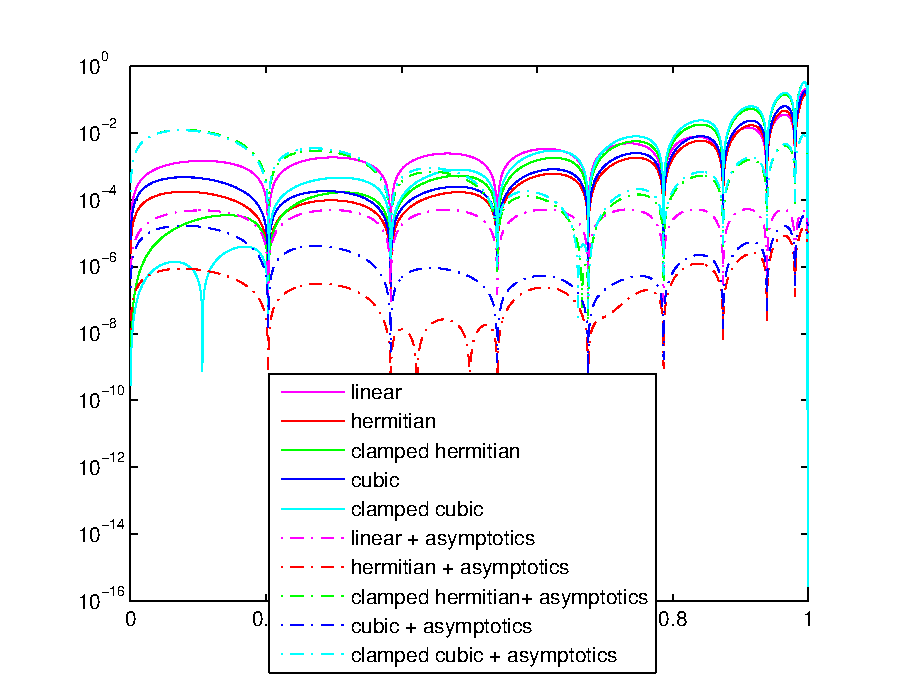
\includegraphics[width=\textwidth]{5_Multifracture_numerical/interpolation_tests/crack_interpolation_N_10}
	\end{subfigure}
	\begin{subfigure}{0.45\textwidth}
		\centering
		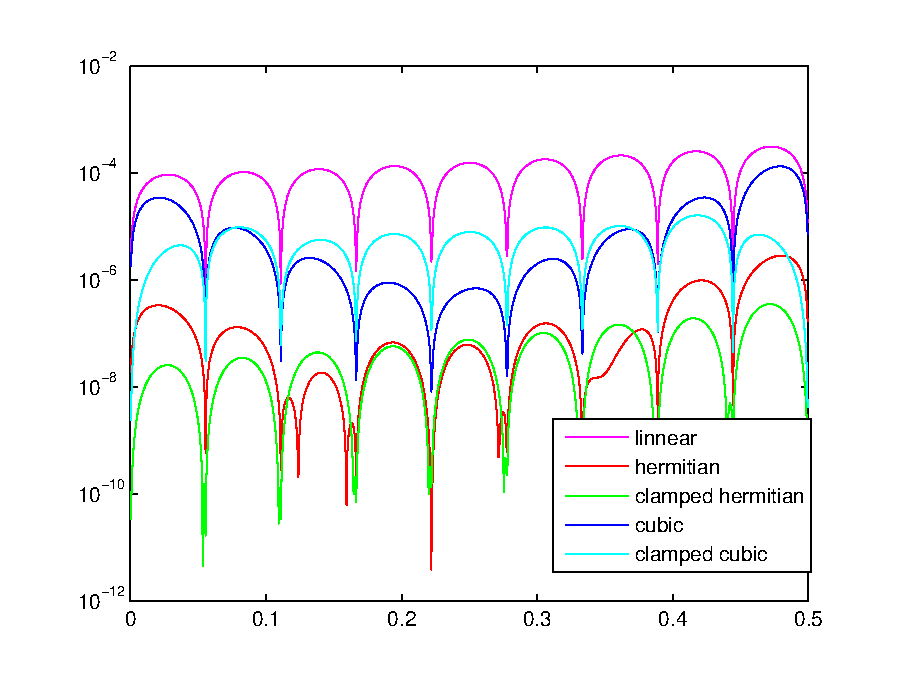
\includegraphics[width=\textwidth]{5_Multifracture_numerical/interpolation_tests/pipe_interpolation_N_10}
	\end{subfigure}
	\caption{Relative error obtained while computing midpoints between $N=10$ points grid, self similar based pipe and crack. First various interpolates were was constructed, then the continuous value of crack and pipe with was approximated.  It is possible to achieve accuracy of $10^-4$ or better for some methods over the entire interval}
\end{figure}